\documentclass[12pt,a4paper]{article}
\usepackage[utf8]{inputenc}
\usepackage{amsmath}
\usepackage{amsfonts}
\usepackage{amssymb}

\usepackage{placeins}
\usepackage{cmap} % для кодировки шрифтов в pdf
\usepackage[T1]{fontenc}
\usepackage{hhline}
\usepackage[unicode]{hyperref}
\usepackage{multirow}
\usepackage{array}
\usepackage{amsmath}
\usepackage{bm}
\usepackage{textcomp}
\usepackage[russian]{babel}
\usepackage{graphicx} % для вставки картинок
\usepackage{amssymb,amsfonts,amsmath,amsthm} % математические дополнения от АМС
\usepackage{indentfirst} % отделять первую строку раздела абзацным отступом тоже
% Поля
\usepackage{geometry}
\geometry{left=2cm}
\geometry{right=1.5cm}
\geometry{top=2.4cm}
\geometry{bottom=2.cm}

%%%%%%%%%%%%%%%%%%%%%%%%%%%%%%%     

\linespread{1.5} % полуторный интервал
\frenchspacing




\begin{document}
	
	\begin{titlepage}
		
		\begin{center}
			\begin{large}
				Санкт-Петербургский Политехнический университет\\ Петра Великого\\
				Физико-механический институт\\
			\end{large}
			\vspace{0.2cm}
			Высшая школа прикладной математики и вычислительной физики\\
			
		\end{center}
		
		\vspace{3cm}
		\begin{center}
			\textbf{Отчёт\\ по лабораторной работе №1\\ по дисциплине\\ "Анализ данных с интервальной \\неопределенностью"}
		\end{center}
		
		\vspace{3cm}
		
		\vbox{%
			\hfill%
			\vbox{%
				\hbox{Выполнил студент:}%
				\hbox{\break}
				\hbox{Иванов Андрей Игоревич,}%
				\hbox{группа 5040102$\backslash$20201}%
				\hbox{\break}
				\hbox{\break}
				\hbox{Проверил:}
				\hbox{\break}
				\hbox{к.ф.-м.н., доцент}
				\hbox{Баженов Александр Николаевич}
			}%
		} 
		\vfill
		
		\begin{center}
			Санкт-Петербург, 2023
		\end{center}
	
	\end{titlepage}
	\tableofcontents
	\newpage
	
	\listoffigures
	\newpage
	
	\section{Постановка задачи}
            Даны две вещественные выборки $X_{+}, X_{-}$. Необходимо:
            \begin{itemize}
                \item Сформировать интервальные выборки $\mathbf{X_{+}}, \mathbf{X_{-}}$;
                \item Реализовать алгоритм вычисления индекса Жаккара;
                \item Найти оптимальный корректирующий множитель $R_{opt}$ такой, что выборка $\mathbf{X_{+}} \cup R_{opt} \cdot \mathbf{X_{-}}$ была наиболее совместной в смысле индекса Жаккара;
                \item Реализовать алгоритм поиска моды выборки;
            \end{itemize}
	\newpage
	
	\section{Теория}
            \subsection{Интервальная выборка}
                Формирование выборки происходит следующим образом:\\
                Пусть $X$ - выборка вещественных чисел. Тогда соответствующая интервальная выборка $\mathbf{X}$ определяется как:
                \begin{equation}
                    \mathbf{X} = \{(x_i - \delta; x_i + \delta)|x_i \in X, i \in \overline{1, |X|}, \delta = \frac{1}{2^{14}}\}
                \end{equation}
            \subsection{Индекс Жаккара}
                Степень совместности двух интервалов $x$ и $y$ может быть определена как коэффициент Жаккара:
                \begin{equation}
                    JK(x, y) = \frac{wid(x \wedge y)}{wid(x \vee y)}
                \end{equation}
                где $\wedge$ и $\vee$ — операции взятия минимума и максимума по включению в полной интервальной арифметике Каухера. Для данной меры совместности справедливо:
                \begin{equation}
                    -1 \leq JK(x, y) \leq 1
                \end{equation}
                Введенная числовая характеристика $JK(x, y)$ может быть естественным образом обобщена на случай интервальной выборки $X = \{x_k\}^n_{k=1}, k = \overline{1,n}$ для определения
                ее меры совместности
                \begin{equation}
                    JK(X) = \frac{wid(\bigwedge_k x_k)}{wid(\bigvee_k x_K)}
                \end{equation}
                Выражение индекса Жаккара можно переписать используя операции взятия минимума
                и максимума в соответствии с определением ширины интервала в классической
                интервальной арифметике:
                \begin{equation}
                    JK(X) = \frac{min(\overline{x_k}) - max(\underline{x_k})}{max(\overline{x_k}) - min(\underline{x_k})}
                \end{equation}

            \subsection{Оптимальный корректирующий множитель}
                Для нахождения $R_opt$ необходимо получить нижнюю и верхнюю границы для последующего уточнения:
                \begin{equation}
                    \underline{R} = \frac{min(\underline{x_i})}{max(\overline{x_i})}
                \end{equation}
                \begin{equation}
                    \overline{R} = \frac{max(\underline{x_i})}{min(\overline{x_i})}
                \end{equation}
                Уточнение $R_opt$ производится либо итерационно с заданным шагом, либо методом половинного деления. Ввиду лучшей скорости для уточнения был использован метод половинного деления, для наглядного отображения зависимости величины $R_{opt}$ от индекса Жаккара использовался итерационный способ с шагом $\frac{wid(\bigcup X)}{100}$.
	\newpage
	
	\section{Реализация}
		Лабораторная работа выполнена на языке Python 3.10 с помощью загружаемых пакетов NumPy и MatPlotLib. Исходный код лабораторной работы находится на \href{https://github.com/Drusiand/SPbSTU_Interval_Analysis.git}{GitHub репозитории}.
	\newpage
	
	\section{Результаты}
		\subsection{Выборка $X_+$}
                \begin{figure}[h!]
                    \centering{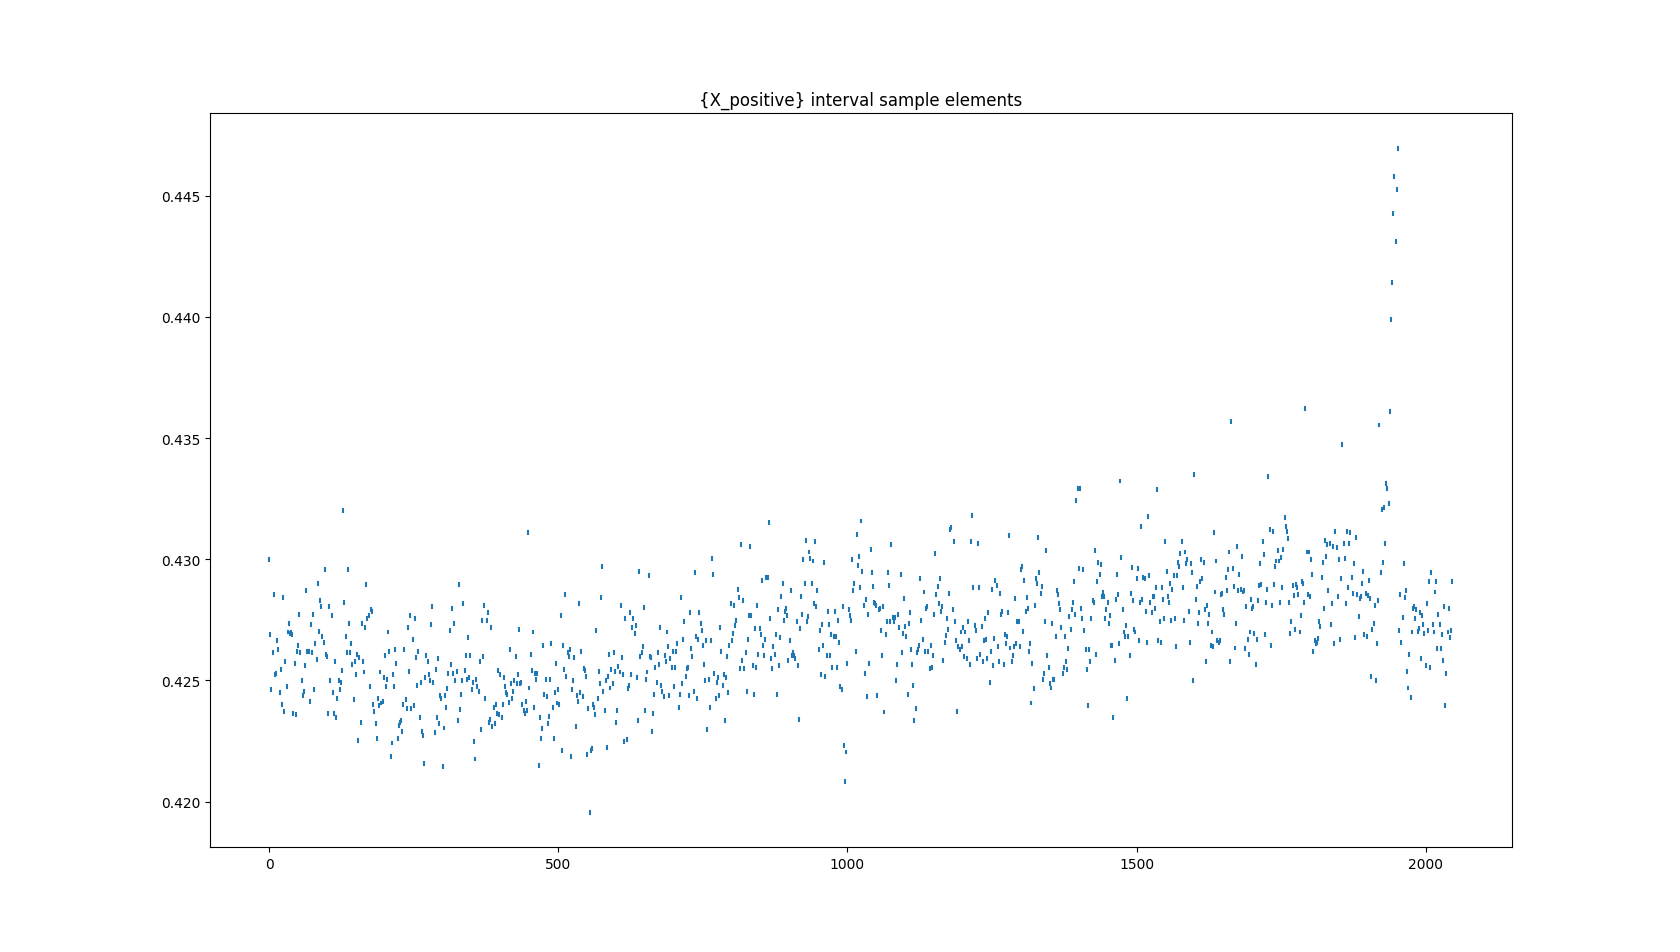
\includegraphics[width=0.95\linewidth]{x_pos.png}}
                        \caption{График интервальной выборки}
                \end{figure}
        	\FloatBarrier
         
                \begin{figure}[h!]                            
                        \centering{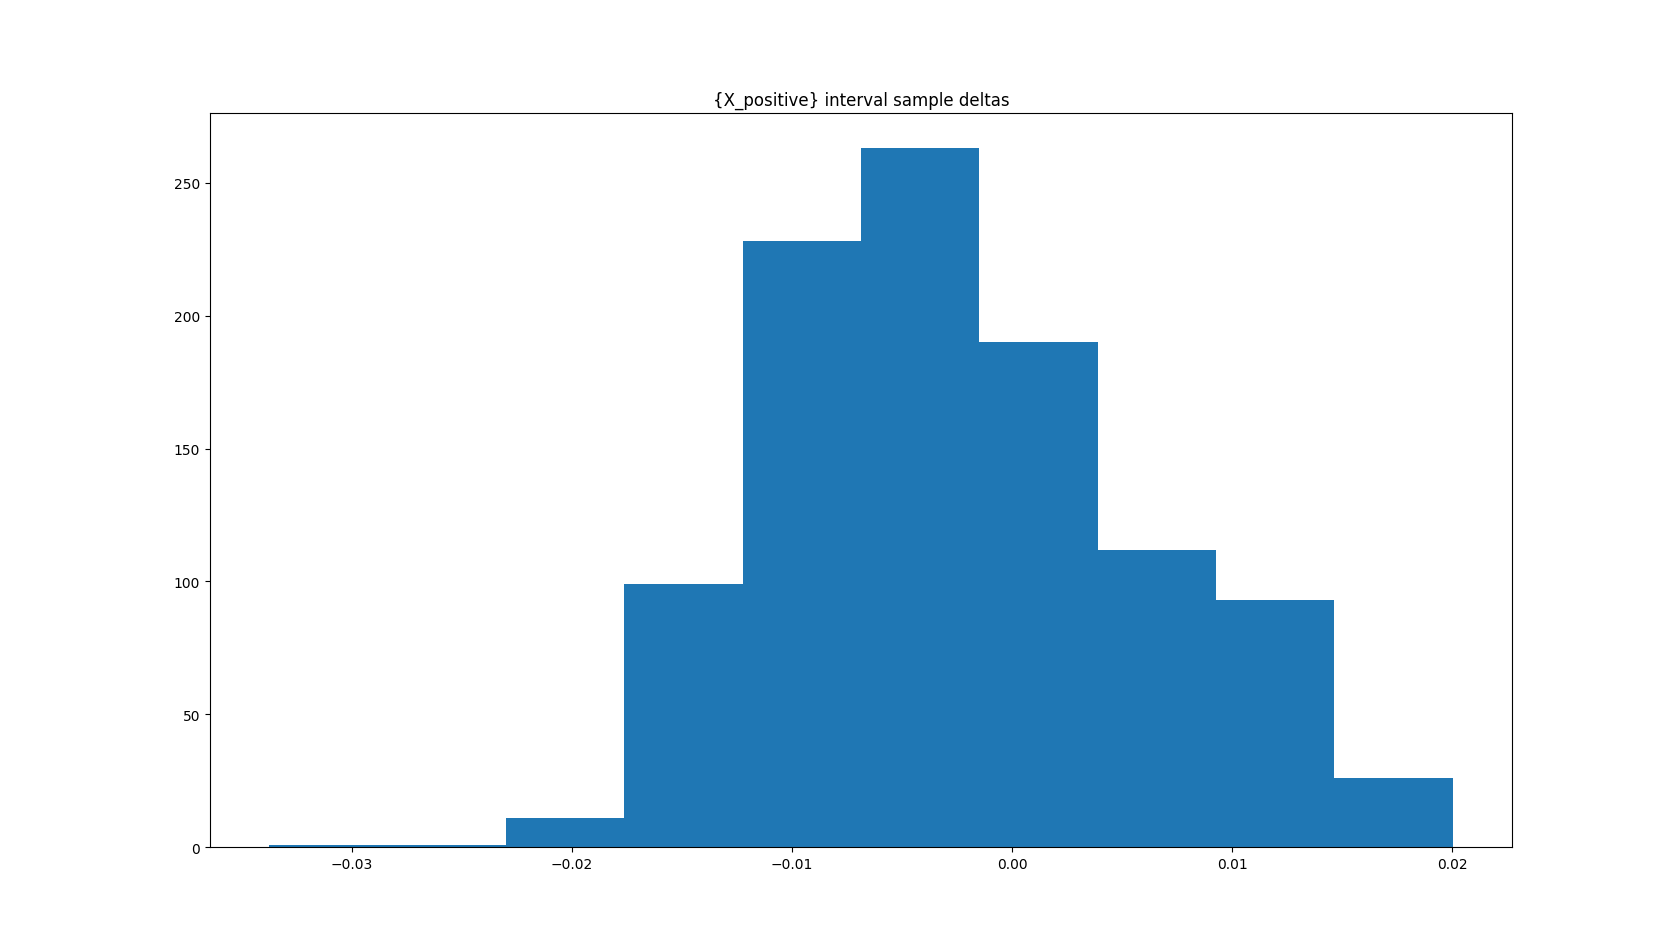
\includegraphics[width=0.95\linewidth]{x_pos_eps.png}}
                        \caption{Гистограмма отступов}
                \end{figure}
        	\FloatBarrier
         
                \begin{figure}[h!]
                    \centering{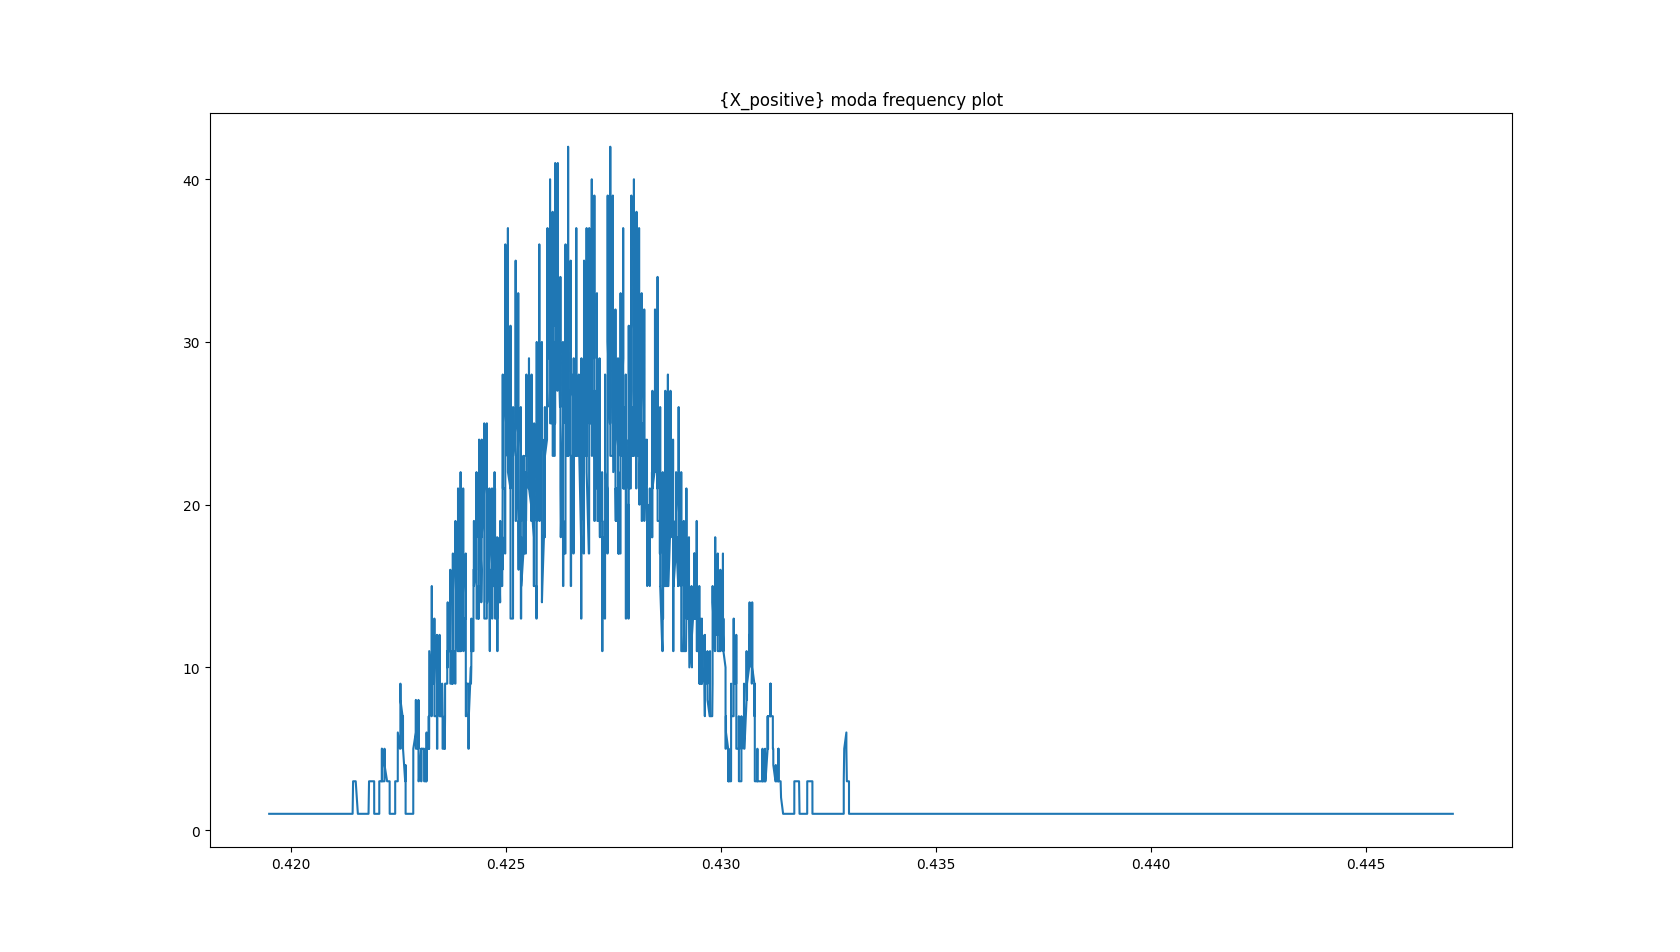
\includegraphics[width=0.95\linewidth]            {x_pos_moda.png}}
                        \caption{График частоты моды}
                \end{figure}
                \FloatBarrier
                
                Данные для формирования интервальной выборки $X_+$ были считаны из файлов 
                \begin{itemize}
                    \item +0\_5V\_4\_.txt
                    \item ZeroLine\_4.txt
                \end{itemize}
                Мода выборки: [0.42645, 0.42743]\\
                На показаниях с порядковым номером в районе 1950 наблдюаются выбросы.
            
		\subsection{Выборка $X_-$}
                \begin{figure}[h!]
                    \centering{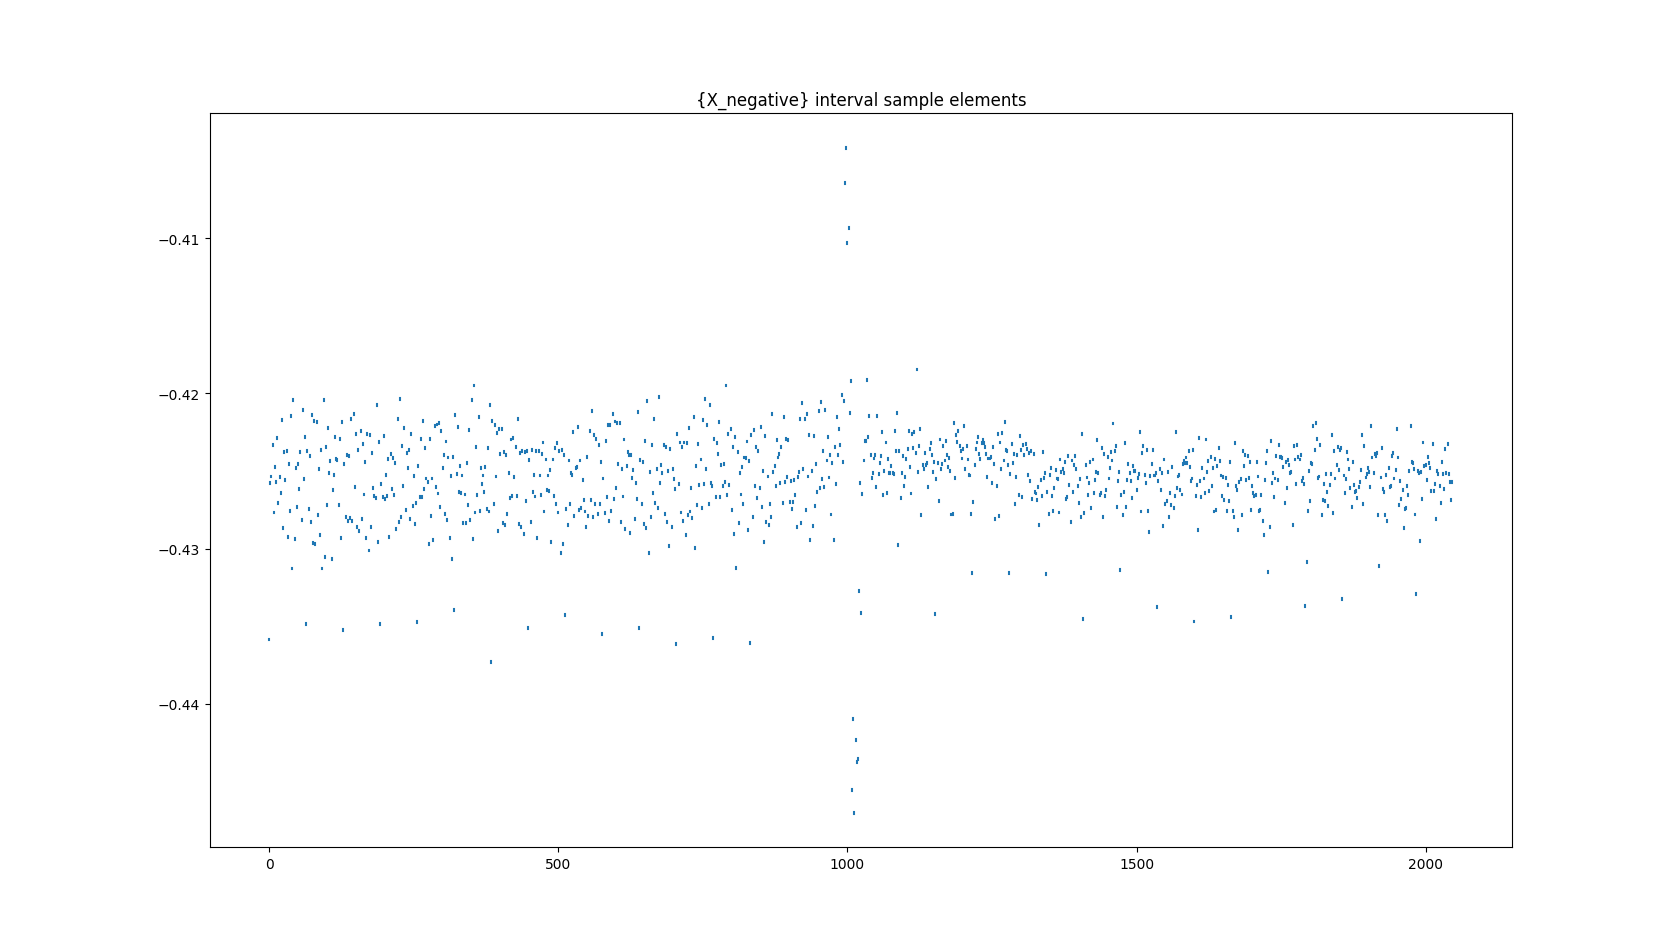
\includegraphics[width=0.95\linewidth]{x_neg.png}}
                        \caption{График интервальной выборки}
                \end{figure}
                \FloatBarrier
                
                \begin{figure}[h!]                            
                        \centering{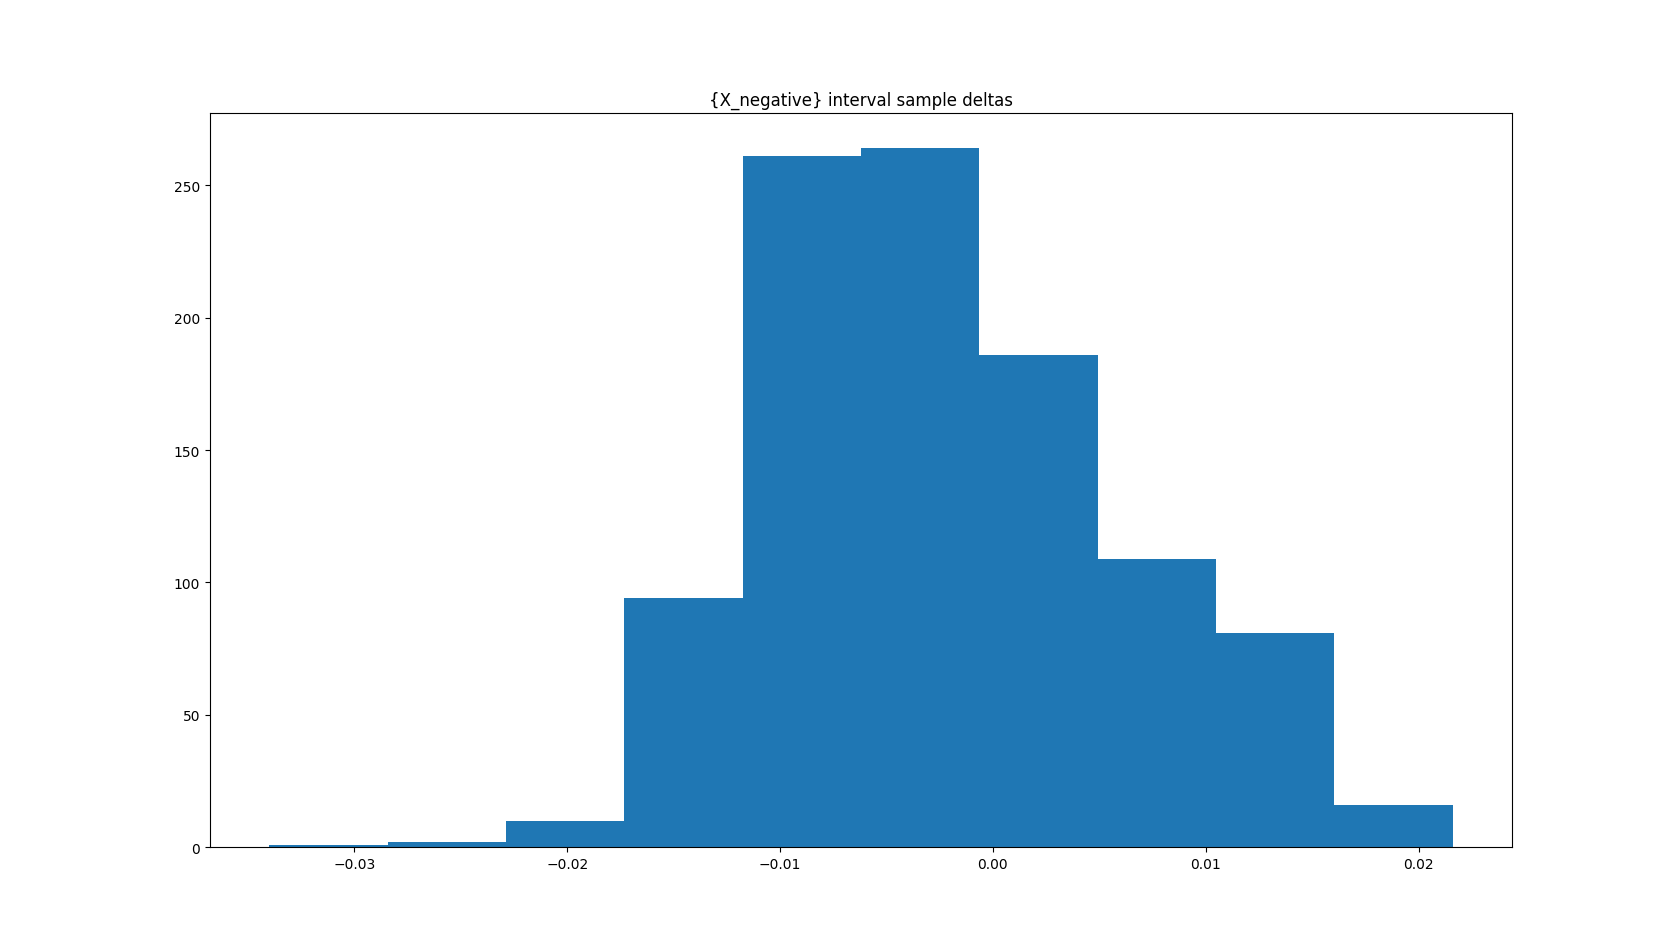
\includegraphics[width=0.95\linewidth]{x_neg_eps.png}}
                        \caption{Гистограмма отступов}
                \end{figure}
                \FloatBarrier
                
                \begin{figure}[h!]
                    \centering{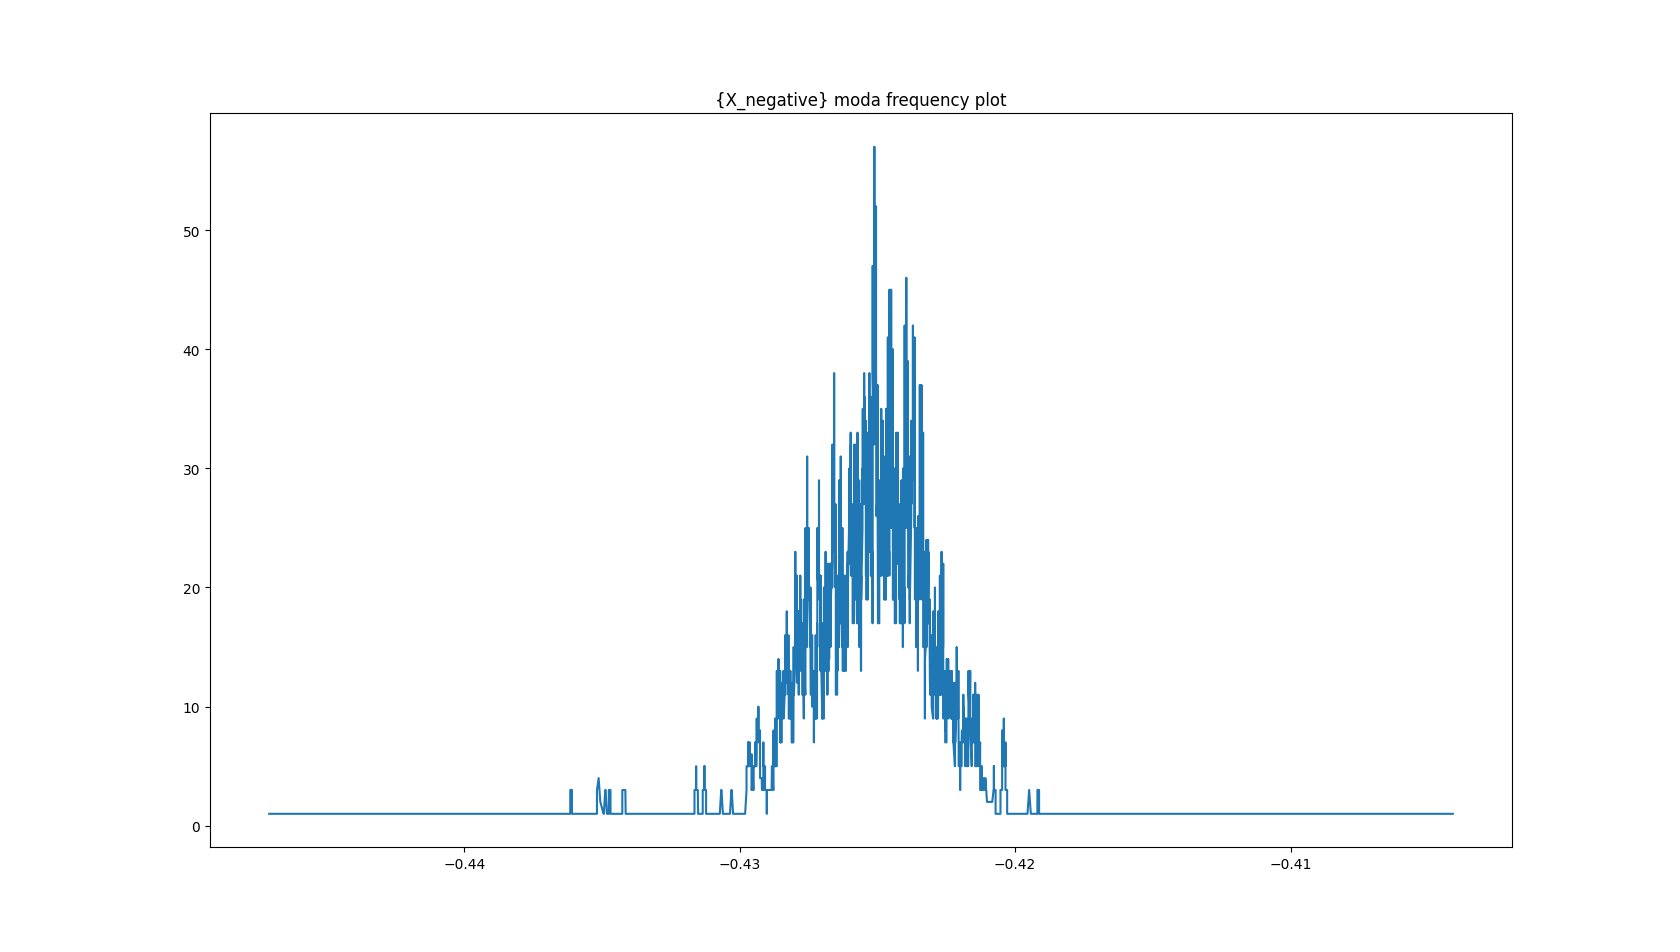
\includegraphics[width=0.95\linewidth]            {x_neg_moda.png}}
                        \caption{График частоты моды}
                \end{figure}
                \FloatBarrier

                Данные для формирования интервальной выборки $X_+$ были считаны из файлов 
                \begin{itemize}
                    \item -0\_5V\_8\_.txt
                    \item ZeroLine\_8.txt
                \end{itemize}
                Мода выборки: [-0.42511, -0.42511]\\
                На показаниях с порядковым номером в районе 1000 наблюдаются выбросы.

                
            \subsection{Поиск корректирующего множителя $R_{opt}$}
                \begin{figure}[H!]
                    \centering{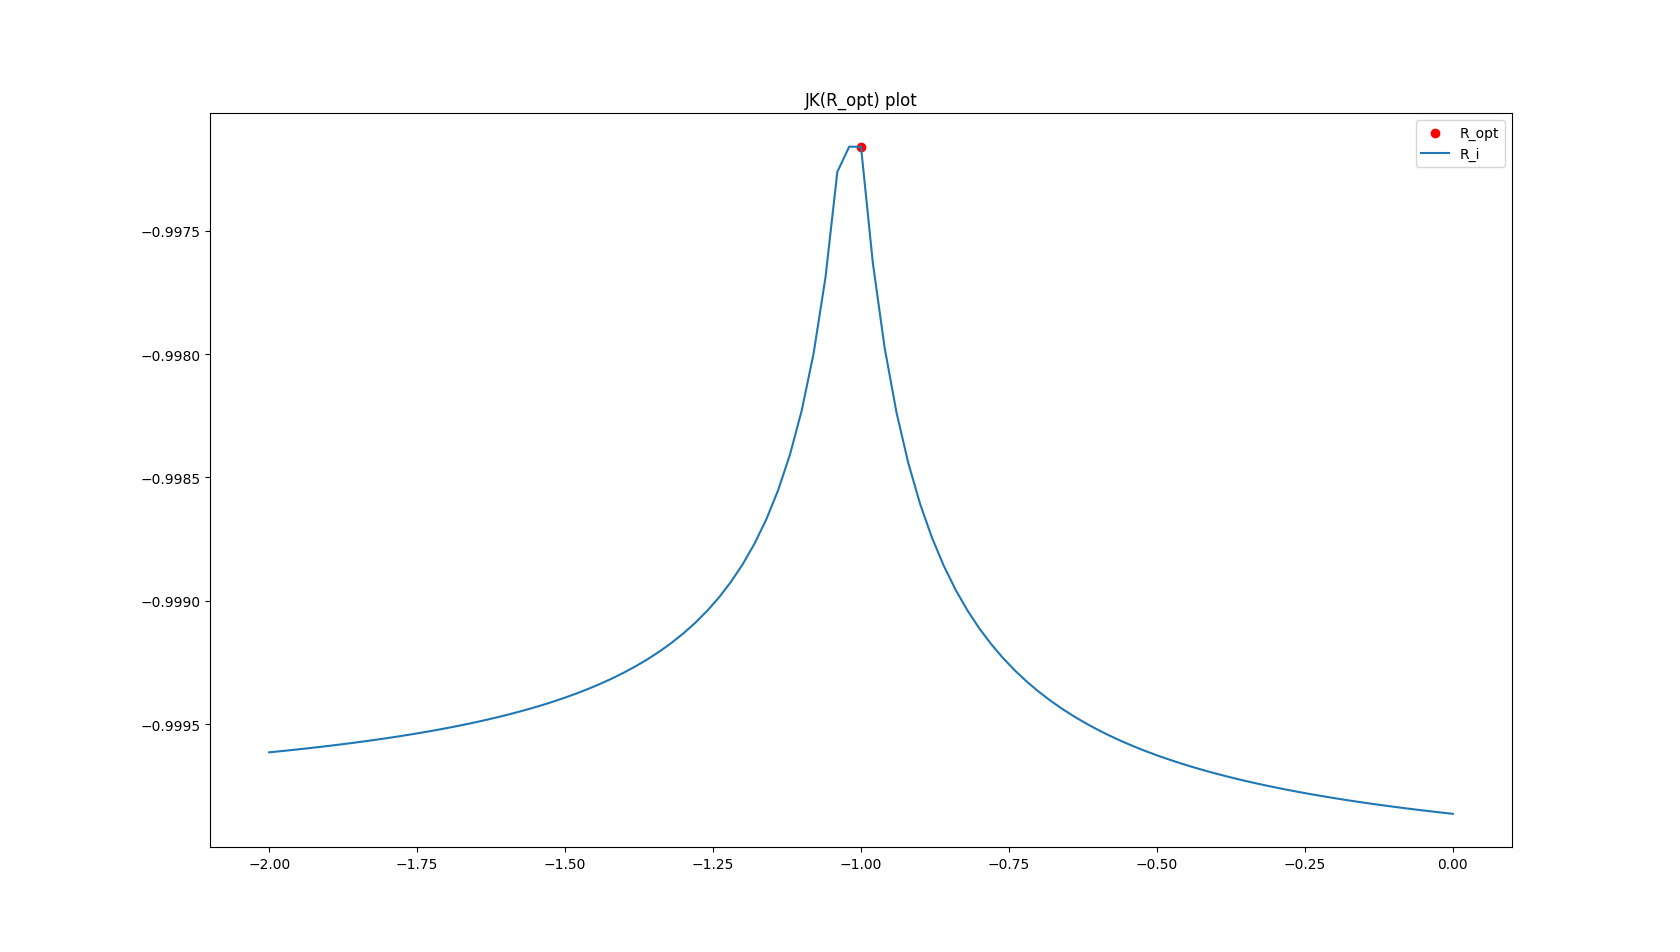
\includegraphics[width=0.95\linewidth]            {R_opt.png}}
                        \caption{График зависимости $JK(X)$ от $R_{opt}$}
                \end{figure}
                
                Было получено значение корректирующегомножителя
                \begin{equation}
                    R_{opt} = -1.0000042926186499
                \end{equation}
                с соответствующим индексом Жаккара:
                \begin{equation}
                    JK(X_+ \cup R_{opt} \cdot X_-) = -0.9971593104169201
                \end{equation}
                                \FloatBarrier

		\subsection{Выборка $X_+ \cup R_{opt} \cdot X_-$}
                \begin{figure}[h!]
                    \centering{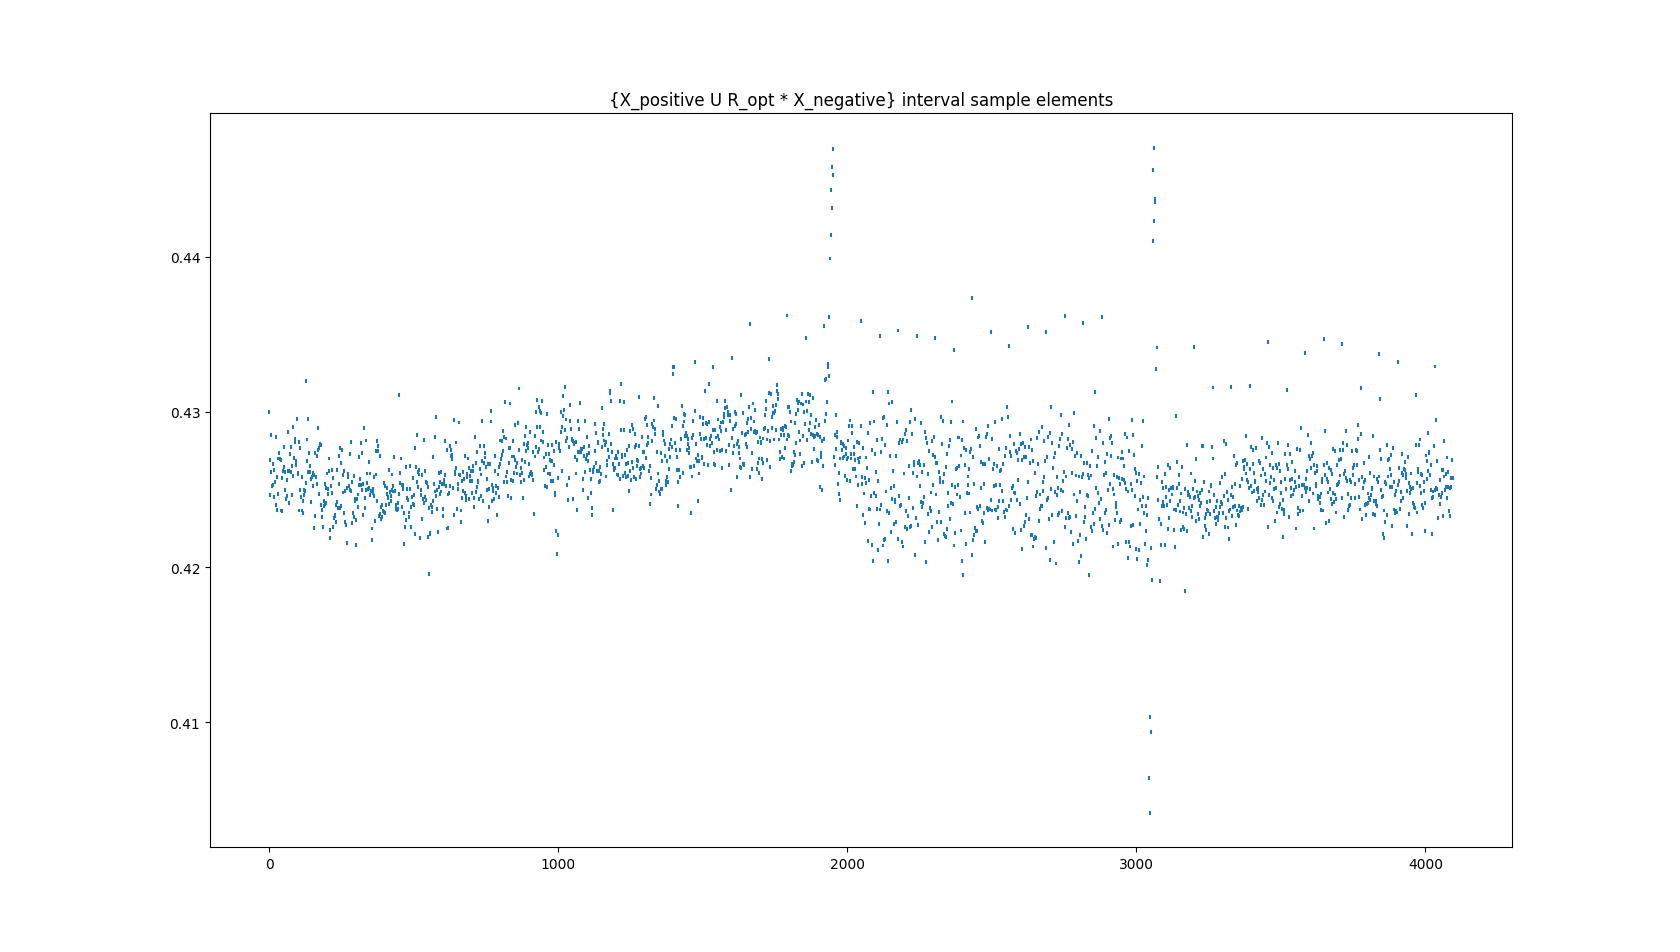
\includegraphics[width=0.95\linewidth]{x_corrected.png}}
                        \caption{График интервальной выборки}
                \end{figure}
                \FloatBarrier
                
                \begin{figure}[h!]
                    \centering{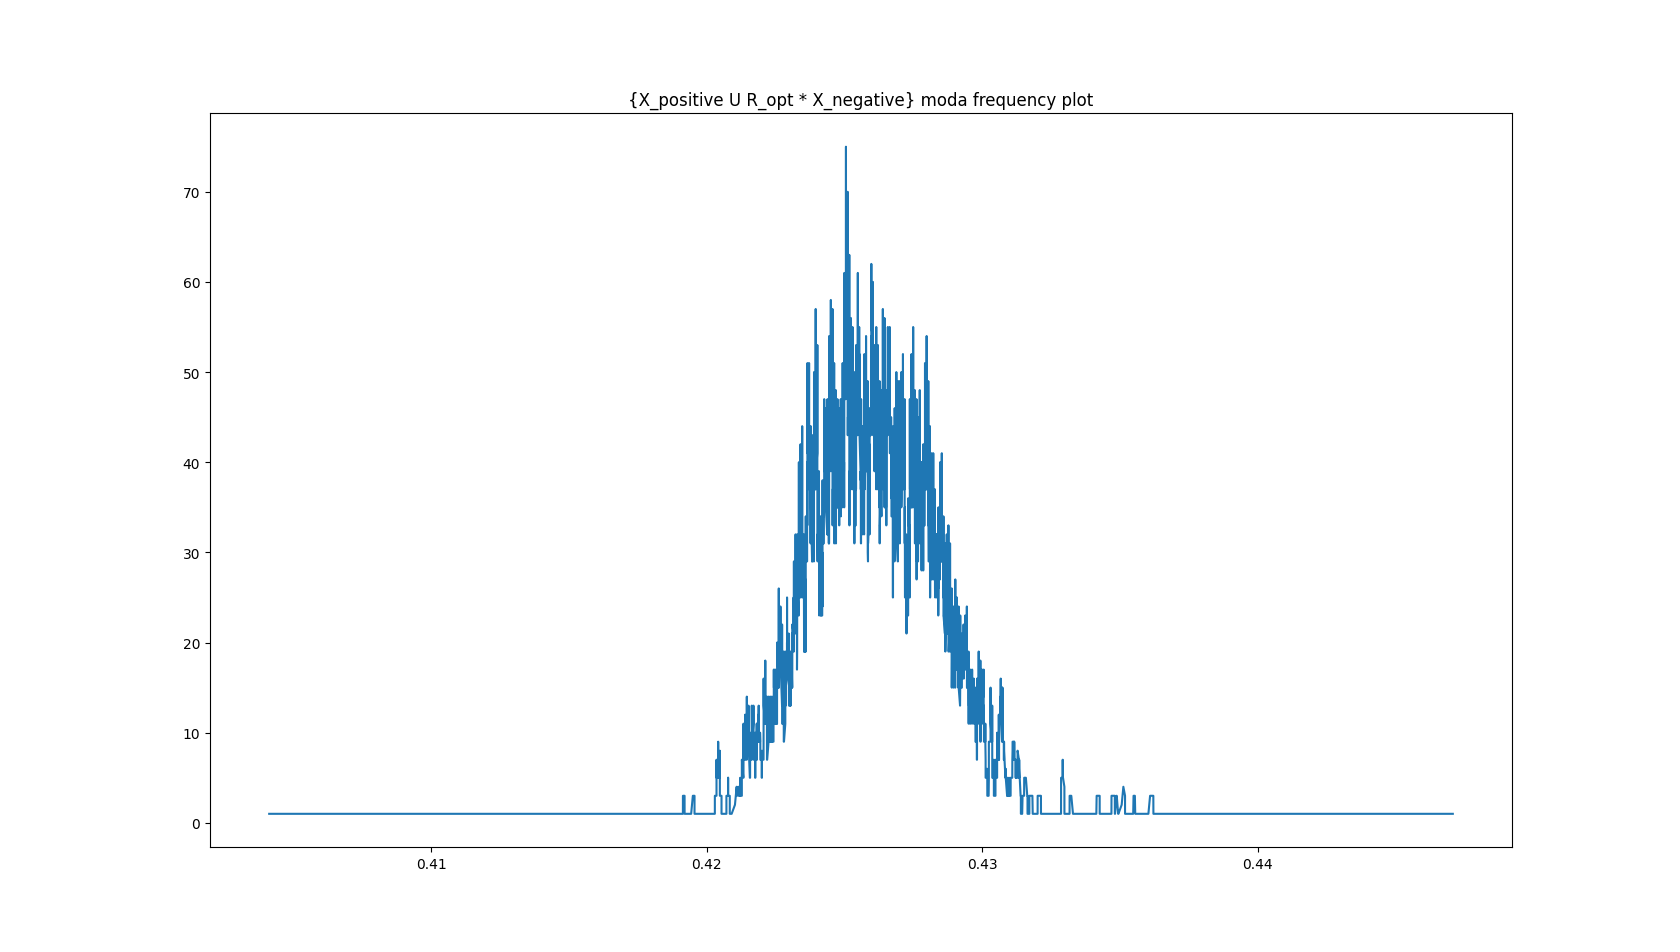
\includegraphics[width=0.95\linewidth]            {x_corrected_moda.png}}
                        \caption{График частоты моды}
                \end{figure}
                \FloatBarrier
      
        \clearpage
	\newpage		
\end{document}